
\section{Introduction}
\label{sec:longitudinal:introduction}
The open publishing model of the web leads to a far faster turnover of documents compared to most conventional printed sources.  In addition, the lifespan of a document is controlled by its author, rather than by any publishing party, often requiring the continuous provision of funds merely to stay available.  The natural conclusion of this is that documents available online are there in a transient, time-limited sense only --- in order to uniquely identify a document online, both a URI and time are needed.

The phenomenon of documents becoming unavailable over time, known as `link rot', has been studied at length by those who seek to index the web, most notably search engine designers.  Lately work has also been done to identify flaws in the longevity of scholarly collections \td{cite "Scholarly context not found"}.

Document change over time also has important ramifications for those working with web data.  Aside from changes in owernship of domain names and site restructuring, many web pages undergo gradual revision and updates, particularly those in the news genres.  Again, whilst there has been study of these events for the purposes of crawler design, the linguistic impact is less known.

Current crawler design (and thus the contents of search engine indices) focuses on keeping the most current page at any given time.  This may be insufficient for many scientific purposes, which must know the context and contents of each page over time, and do so in a manner comparable to other documents from that time period.

This chapter starts with...
\til{signposting}


\section{Document Attrition}
\label{sec:longitudinal:attrition}

% FIXME Does this belong in the lit review?
\section{Review of Current Use}
Here I'll discuss current usage of WaC work, and focus on why attrition is likely to be important to CL in general.  This will serve part of the rationale of this chapter.

\subsection{Methods for Sampling Web Data}
I intend to cover methods people use for sampling.  This will include all the various tools (and commentary on each, though there will likely not be time for an evaluation of each).  From this, various deficiencies will be extracted, which will form the basis for my improved tools.


% --------------- %
\section{Re-Implementation of Sharoff's Paper}
This will form, basically, a motivating example for the incomparability of results taken years apart from the web.



\section{Comprehensive DA Study}
The content from my longitudinal study will fall here, though it's possible to populate some of this will LREC and other work.

\subsection{Method}
In addition to a discussion of best practice (perhaps best moved elsewhere?), outline the study:
\begin{itemize}
	\item The process of sampling, related to the lit review;
	\item The choice of input data.
\end{itemize}


\subsection{Evaluation \& Analysis}
Analyse the results, and provide an evaluation of:
\begin{itemize}
	\item The study itself, and the quality of its findings;
	\item The impact any identified effects are likely to have upon data integrity.
\end{itemize}






\section{LWAC: Longitudinal WaC Sampling}
\label{sec:longitudinal:lwac}


\subsection{Rationale}

Many sampling efforts for linguistic data on the web are heavily focused on producing results comparable to conventional corpora.  These typically take two forms: those based on URI lists (e.g. from search results, as in %~\cite{sharoff2006creating}
BE06~\cite{baker2009be06}, BootCat~\cite{baroni2004bootcat}), and those formed through crawling (e.g. enTenTen\footnote{\url{http://trac.sketchengine.co.uk/wiki/\\Corpora/enTenTen}}, %~\cite{}, %FIXME
UKWaC~\cite{ferraresi2008introducing}).

Though initial efforts in web-as-corpus (WaC) focused on the former method %, in part due to concerns over the balance of samples returned, 
many projects are now constructing supercorpora, which may themselves be searched with greater precision than the `raw' web, in line with Kilgarriff's vision of linguistic search engines~\cite{kilgarriff2003linguistic}.  This has led to the proliferation of crawlers such as those used in~\cite{schafer8building} and WebCorp\footnote{\url{http://www.webcorp.org.uk/live/
}}~\cite{renouf2003webcorp}.

% diachronic work with webcorp.
% \cite{kehoe2006diachronic}
% \cite{kehoe2009weaving}

This approach, with its base in a continually-growing supercorpus, parallels the strategy of a monitor corpus~\cite{sinclair1982monitor}, and is applicable to linguistic inquiry concerned with diachronic properties~\cite{kehoe2006diachronic}.
%Even for informal searches, tools for date-based lookup are increasingly (e.g. Google).


Repeated sampling by crawling, whilst balanced linguistically, omits subtler technical aspects that govern consumption of data online, most notably the user's impression of its location, as defined by the URI.  Low publishing costs online, paired with increasing corporate oversight and reputation management (both personal ~\cite{ICT4DBibliography1650} 
and professional~\cite{Malaga2000repman})), have lead to a situation where this content is being revised frequently, often without users even noticing.

The nature of within-URI change have been studied from a technical perspective by those interested in managing network infrastructure, compiling digital libraries~\cite{tyler2003librarians}, and optimising the maintenance of search engine databases~\cite{koehler2004longitudinal}.  The needs of these parties are quite aside from those of corpus researchers, however, since they focus around a best-effort database of information, rather than a dependable longitudinal sample with known margins for error.

% ---
Current methods for sampling language change online include:

\begin{itemizeTitle}

    \item[Crawlers/Revisiting] Continuously crawl pages, adding new ones as links are updated and revisiting old ones according to heuristics;
    \item[Diachronic corpora] Build two separate corpora using the same sample design at different points in time;
    \item[Monitor corpora] Continuously add new material to a corpus as it is created, agnostic of change;
    \item[Subsampling supercorpora] Build a large corpus and select documents from it according to a bimodal distribution of document age;
    \item[Feed corpora] Crawl pages on publication date (a form of monitor corpus).

\end{itemizeTitle}


Each of these methods is subject to a number of downsides, making them difficult to use for many scientific purposes, or requiring significant resources and forward-planning (thus putting them out of the hands of most researchers).  Some issues, such as irregular revisiting of pages and the lack of detail stored about network-level metadata, complicate the process of analysis.  Most corpus formats are also not annotated by time, meaning that analysis often requires repeated export and comparison --- tools for which must be produced on a case-by-case basis.

% 
% \begin{itemize}
%     \item \textsl{Incremental sampling}---Search engine databases and digital archives are persistent, and may be incrementally updated in a continuous manner whilst still being useful;
%     \item \textsl{Lack of comparability}---A cross-sectional sample of search databses yields documents sampled at various times, with a possible age variation as modelled by the specific type of web page.  This is evidenced well by the relative likelihood of receiving a broken link when searching for current events \textsl{vs.} older scientific articles.
%     \item \textsl{Information-seeking behaviour}---Search engine literature indicates [CITE] that information, when lost from one location, is often available at many others.  This same process is unlikely to be followed, however, if a resource has simply changed, or if a user relies on a small set of web pages as an information resource (such as news sources).
%     \item \textsl{Deliberate `usefulness bias'}---Sources deemed to be pertinent to a search engine's clientelle are sampled more frequently, and thoroughly.  This results in persistence-of-value surrounding high-profile domain names and companies, which dominate the zipfian distribution of web results.
% \end{itemize}
% 


We present here a tool, LWAC, for this form of longitudinal sampling, designed to maximise the comparability of documents downloaded in each sample in terms of their URI rather than content.  To accomplish this, we use a cohort sampling strategy, as illustrated in Figure~\ref{fig:longitudinal:lwac:samples}, to get full coverage over a list of URIs, at the expense of sampling new content.

\begin{figure}[Ht]
    \centering
    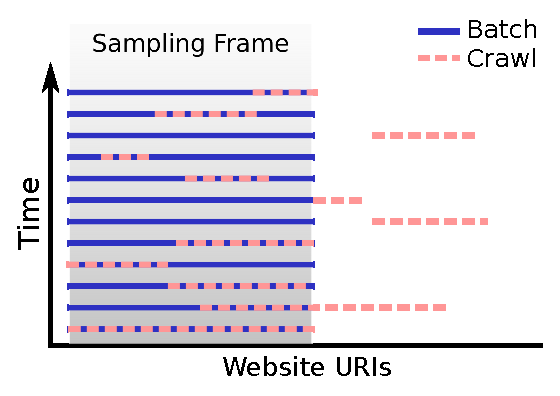
\includegraphics[width=0.8\textwidth]{longitudinal/lwac-samples}
    \caption{URI coverage for batch and crawl}
    \label{fig:longitudinal:lwac:samples}
\end{figure}

This approach allows for reliable re-visits to each member of the sample, and thus the construction of vertically comparable data points, whilst making short-term effects visible by revisiting each link.  Such a sample design should repeat each individual sample as quickly as possible, so as to minimise the time differences between documents within.

\til{Continue writing up `LWAC' slides from here}


\section{Applications}
Our strategy allows us to investigate how language may change in relation to technical and social events in a way that mimics the experience of the end user, and offers a useful perspective on many epistemic problems of WaC methods, to determine:

\begin{itemize}
    \item The portions of web pages that typically change as main content regions;
        \vspace{-6pt}
    \item The impact of social feedback and user generated content on page content;
        \vspace{-6pt}
    \item How censorship, redaction and revision affect website contents;
        \vspace{-6pt}
    \item Website resource persistence and its relation to linguistic content (link rot/document attrition);
        \vspace{-6pt}
    \item How institutions' publishing policies affect reporting of current events.
\end{itemize}

In order to maximise its coverage of these topics, LWAC~is designed to construct longitudinal samples from arbitrary URI lists, using commodity hardware, in a way that mimics the user's experience of a website.  


% The tool is designed to construct longitudinal samples from URI lists, using only commodity hardware.  It is designed with `full storage' in mind, that is, recording everything about each HTTP session in such a way that it may later be exported and accessed in a parsimonious manner.







\subsection{Design \& Implementation}


\begin{figure}[Ht]
    \centering
    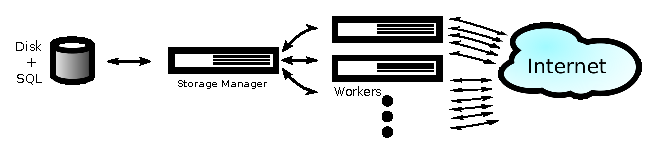
\includegraphics[width=0.8\textwidth]{longitudinal/lwac-arch}
    \caption{System Architecture}
    \label{fig:longitudinal:lwac:arch}
\end{figure}

In order to form a useful longitudinal sample, each data point should be as time-invariate as possible.  As such, a highly parallel, distributed architecture was selected (Figure~\ref{fig:longitudinal:lwac:arch}).  This yields technical benefits in terms of throughput (especially where the internet connection is a bottleneck), flexibility, and the ability to differentiate between websites that are blocked for a given area of the internet and those that are offline proper.

Data storage in the system is split between metadata, stored in an SQL database, and website sample data itself, which is stored as raw HTTP response data in a versioned structure on disk.  The storage format is optimised for large samples, and is nested in order to avoid common filesystem limits.  LWAC~does not enumerate URIs in memory, meaning there is no hard limit on corpus size.

The download process is managed by a central server, which co-ordinates storage and metadata access and provides full atomicity.  This server distributes batch jobs, according to policies governing reliability and throughput, to worker clients, which compete for the opportunity to download web pages.

Workers are able to imitate the behaviour of end users' browsers as much as possible, so as to avoid search engine optimisation and user-agent detection tactics (for example, they may retain cookies and present typical request headers).

After downloads have occurred, data may be retrieved for analysis in a variety of formats using the included export tool.






\subsection{Performance}


\subsection{Summary}







\section{Summary}
\label{sec:longitudinal:summary}
Mention which of these are to be selected and why, link to later chapters.
